
\begin{frame}
    \frametitle{Sistemas Distribuidos - Modelos de Replicación}

    Una de las características de los sistemas NoSQL es la facilidad de correr en sistemas distribuidos, lo que permite el escalado horizontal.

     

    Generalmente se realiza cuando el sistema está operativo.

     
    
    Se necesitan técnicas para distribuir la información actual entre los nuevos nodos sin interrumpir al sistema.

     

    Para resolver este problema están los 
    
    \begin{center}
        \textbf{Modelos de Replicación}
    \end{center}

     

    Los dos principales son \textbf{Maestro-Esclavo} y \textbf{Maestro-Maestro}
    
\end{frame}

\begin{frame}
    \frametitle{Sistemas Distribuidos - Modelo Maestro-Esclavo}

    En este modelo tenemos un \textbf{Maestro} y uno o más \textbf{Esclavos}.

     

    \begin{itemize}
        \item \textbf{Maestro.}
        
        \begin{enumerate}
            \item Es el nodo principal del sistema.
            \item Responsable de aceptar escrituras en la base de datos.
        \end{enumerate}
        
         

        \item \textbf{Esclavo.} 
        
        \begin{enumerate}
            \item Es un nodo secundario del sistema.
            \item Se sincroniza con el maestro para mantener una copia de los datos. 
            \item Solo acepta lecturas.
        \end{enumerate} 
    \end{itemize}

     

    \begin{center}
        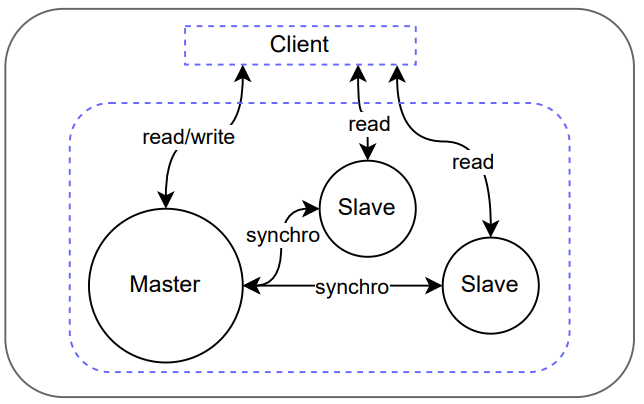
\includegraphics[width=0.5\textwidth]{diagramas/maestro-esclavo.png}
    \end{center}
    
\end{frame}

\begin{frame}
    \frametitle{Sistemas Distribuidos - Modelo Maestro-Maestro}

    En este modelo todos los nodos en el sistema son tanto \textbf{Maestros} como \textbf{Esclavos}.

     

    La replicación de datos es bidireccional.

     

    Cada nodo es responsable de mantener una copia exacta de los datos y asegurar la sincronización.

     

    \begin{center}
        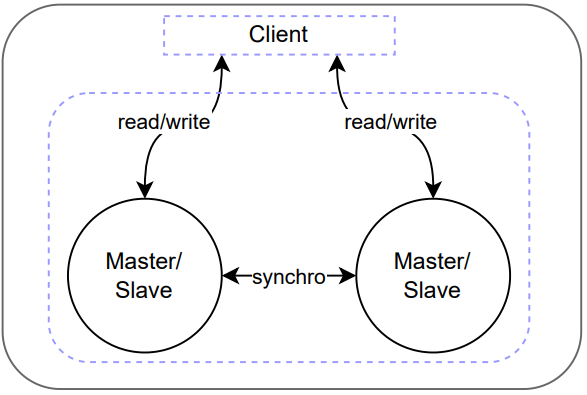
\includegraphics[width=0.5\textwidth]{diagramas/maestro-maestro.png}
    \end{center}
    
\end{frame}

\begin{frame}
    \frametitle{Sistemas Distribuidos - Modelos de Replicación}

    La principal diferencia entre los modelos, es que el modelo \textbf{Maestro-Esclavo} cuenta con un único nodo \textbf{Maestro}.

     

    Por lo que podemos decir que dicho modelo cuenta con un control \textit{Centralizado}.

     

    Este nodo se puede convertir en un cuello de botella.   Y además, si falla el nodo Maestro...   estamos en problemas.

     

    Igualmente, existen soluciones para este problema 
    
    \begin{enumerate}
        \item Tener uno o más nodos Maestros de backup.  
        \item Asignar hardware potente al nodo Maestro.  
        \item etc.
    \end{enumerate}

     

    Estas soluciones pueden combinarse.
    
\end{frame}

\begin{frame}
    \frametitle{Sistemas Distribuidos - Partición de Archivos}

    La Partición de Archivos es otra característica a tener en cuenta en los sistemas distribuidos.

     

    Se refiere a la división de la información en fragmentos que se distribuyen entre los nodos.

     

    Esta distribución mejora el rendimiento al permitir a su vez distribuir las consultas y hacer paralelismo. 

     

    Aumenta la resilencia del sistema debido a la redundancia de la información, si falla algún nodo, la información sigue disponible.
    
\end{frame}

\begin{frame}
    \frametitle{Sistemas Distribuidos - Acceso de Datos de Alto Desempeño}

    Generalmente se necesita encontrar un registro particular entre millones.

     

    El crecimiento de la información hace que esta búsqueda se ralentice.

     

    Aquí entra en juego el \textit{High Performance Data Access} (HPDA).

     

    Se refiere a la capacidad de un sistema para acceder y manipular grandes volúmenes de datos de manera rápida y eficiente.

     

    Se suelen utilizar técnicas de \textit{hashing} y/o particionado de rango sobre claves de valores.
    
\end{frame}

\begin{frame}
    \frametitle{Sistemas Distribuidos - Acceso de Datos de Alto Desempeño}

    \begin{itemize}
        \item \textbf{Hashing.}

        Esta técnica aplica una función de hash $h$ a una clave $K$.

         
    
        La aplicación $h(K)$ devuelve la ubicación del objeto en el sistema distribuido.

         
        
        \item \textbf{Particionado de rango sobre claves.} 

        Se asignan los valores a ubicaciones en función de un rango de valores de clave.

         

        Una ubicación $u$ podría tener los valores cuyas claves $K$ estén en el rango
        
        \begin{center}
            $Ku_{min} \leq K \leq Ku_{max}$
        \end{center}
        
    \end{itemize}
\end{frame}

\begin{frame}
    \frametitle{Sistemas Distribuidos - Conjetura de Brewer}

    También conocida como Teorema CAP.

     
    
    Las siglas \textbf{CAP} vienen de:

     

    \begin{itemize}
        \item \textit{\textbf{C}onsistency} (Consistencia)                        

        \item \textit{\textbf{A}vailability} (Disponibilidad)                     

        \item \textit{\textbf{P}artition Tolerance} (Tolerancia a Particiones)
        
    \end{itemize}

      
    
    Dicho Teorema enuncia lo siguiente

     
    
    \begin{Teorema}
    Dadas las propiedades \textbf{Consistencia}, \textbf{Disponibilidad} y \textbf{Tolerancia a Particiones}, solo se pueden cumplir dos de estas tres simultáneamente en un sistema distribuido.
    \end{Teorema}

     

    Los sistemas NoSQL, sacrifican la consistencia por \textit{consistencia eventual}, para garantizar en mayor medida disponibilidad y tolerancia a particiones.
    
\end{frame}